
    \documentclass[11pt]{article}
    \usepackage{a4wide}
    \usepackage[dvips]{graphicx}
    \newcommand{\printindex}[0]{} %recover pod2latex bug
    \begin{document}
    \begin{center}
        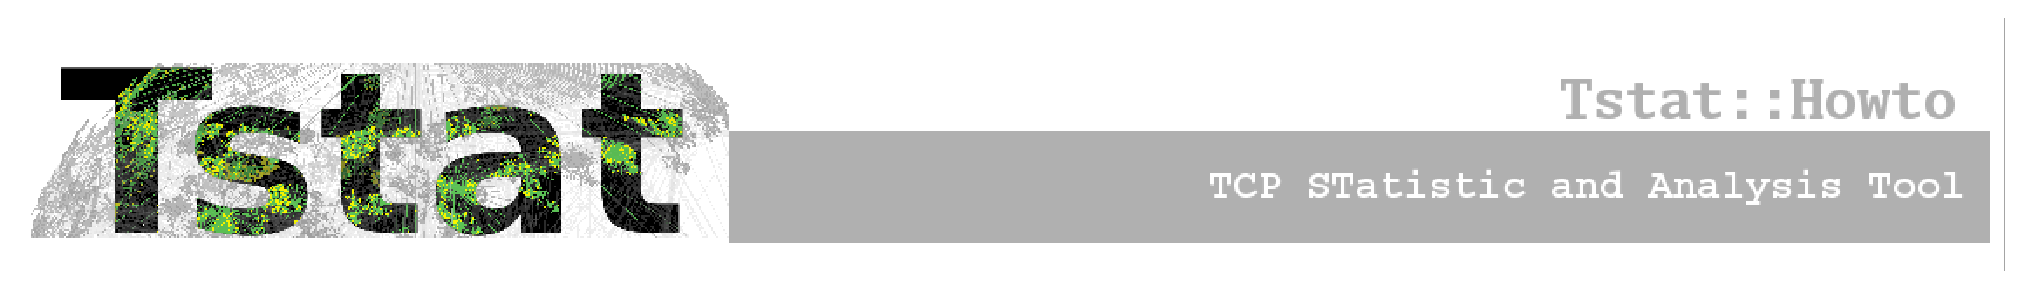
\includegraphics[width=\textwidth]{tstat_banner.eps}
    \end{center}
    \tableofcontents
    
%%  Latex generated from POD in document /home/httpd/html/HOWTO/~HOWTO.pod
%%  Using the perl module Pod::LaTeX
%%  Converted on Thu Jun  9 13:50:03 2005

%%  Preamble supplied by user.

\clearpage

       %palatino
       \fontfamily{ppl}\selectfont


\section{Installation\label{Installation}\index{Installation}}


This document provides basic information
for the installation, configuration and usage 
of Tstat and its optional add-ons.

\subsection{Requirements\label{Requirements}\index{Requirements}}
\subsubsection{Operating System\label{Operating_System}\index{Operating System}}


Tstat has been tested tested on \texttt{Linux 2.2.x}, \texttt{2.4.x} and \texttt{2.6.x} kernels, 
using \texttt{RedHat 6.x-9.x}, and \texttt{Fedora Core x} systems. 
It should work under other \texttt{UNIX} dialects, such as 
\texttt{FreeBSD}, \texttt{NetBSD 1.3} and \texttt{MAC OS X} (although we don't have either of 
those platforms for testing purposes). If you are able to run Tstat on 
other OSs, we'll be happy to include them in the list.

\subsubsection{System Libraries\label{System_Libraries}\index{System Libraries}}


Tstat requires, by itself, a few library that should
already be installed on your system, such as 
\texttt{libpcap} (available from \textsf{http://www.tcpdump.org}) 
or the DAG drivers (available from \textsf{http://www.endace.com}), 
in case you use such hardware. With these libraries, 
you are ready to capture and process the traffic flowing
in your LAN.



Since Tstat uses pthread to improve the performance in case of real time
analysis, your system must support POSIX thread as well.



Finally, to use the RRD functionalities, you also need to have a working
installatin of the RRDtool (available from
\textsf{http://people.ee.ethz.ch/\texttt{\~{}}oetiker/webtools/rrdtool/}).

\subsubsection{Post-Processing\label{Post-Processing}\index{Post-Processing}}


Some of the additional plotting capabilities, such
as the ones used in Tstat's old web interface at
\textsf{http://tstat.tlc.polito.it/tstat.old/}, requires
Perl 5.x and some modules to be installed on your system. 
Both Perl and the required modules (namely, \texttt{Date::Manip}
and \texttt{Compress::Zlib}) are available from \textsf{http://www.cpan.org}.
With these tools, you are ready to perform additional 
post-processing  and visualize the collected dataset.

\subsubsection{Round-Robin Database\label{Round-Robin_Database}\index{Round-Robin Database}}


Finally, weather you plan to use the Round-Robin Database
capabilities featured by Tstat, then you need to install
\texttt{RRDtool} on your system (available from
\textsf{http://people.ee.ethz.ch/\texttt{\~{}}oetiker/webtools/rrdtool/}).
Although Tstat works
with \textit{any} version of RRDtool (we have successfully tried 
with 1.0.x and 1.2.x), you may want to download its latest 
version. With RRDtool, you are ready for extremely-scalable 
traffic monitoring and analysis.

\subsection{Installation Instructions\label{Installation_Instructions}\index{Installation Instructions}}


Download and uncompress the tarball. Assuming
that you want to download version \texttt{1.x}, this can be done with:

\begin{small}\begin{verbatim}
         wget http://tstat.tlc.polito.it/download/tstat-1.x.tgz
         tar xzvf tstat-1.x.tgz
         cd tstat-1.x/
\end{verbatim}\end{small} \noindent
Check the \texttt{Makefile.in} (\textit{double check it!} ;-)), choosing the correct options
you like  based on your system configurations. The changes are very simple, such
as adding or removing supported input file formats and compression tools,
toggling support for DAG (default \texttt{off}), and RRDtool (default \texttt{off}). All the
compile time options are managed via \texttt{\#define} directives.  Now, run:

\begin{small}\begin{verbatim}
        ./configure
\end{verbatim}\end{small} \noindent
to generate a suitable \texttt{Makefile}. Then run:

\begin{small}\begin{verbatim}
         make
\end{verbatim}\end{small} \noindent
to produce an executable file named \texttt{tstat}.



\# For instructions
\#related to the Round Robin Database module installation and
\#configuration, please refer to the Sec.~\ref{RRD_Module}
\#on this document.

\section{Usage\label{Usage}\index{Usage}}


There are few things to know to run Tstat: first, you are required to have a
knowledge  of the network that you want to monitor. 
Second, there are the few options that are described in this section.

\subsection{Synopsis\label{Synopsis}\index{Synopsis}}


Tstat primary usage is as a command-line tool; the synopsis of 
the command is the following:

\begin{small}\begin{verbatim}
       tstat  [-hHtuvwp] [-d[-d]] [-Nfile] [-sdir]
              [-rRRD_out_dir] [-Rrrd_conf] [-S]
              [-l] [-iinterface]
              [-ffilterfile] <file1 file2>
\end{verbatim}\end{small} \noindent
\begin{small}\begin{verbatim}
        -h: print this help and exit
        -H: print internal histograms names and definitions
        -t: print ticks showing the trace analysis progress
        -u: do not trace UDP packets
        -v: print version and exit
        -w: print [lots] of warning
        -p: enable multi-threaded engine (useful for live capture)
\end{verbatim}\end{small} \noindent
\begin{small}\begin{verbatim}
        -d: increase debug level (repeat to increase debug level)
        -Nfile: specify the file name which contains the
                description of the internal networks.
                This file must contain the subnets that will be
                considered as 'internal' during the analysis
                Each subnet must be specified using network IP address
                on the first line and NETMASK on the next line:
                130.192.0.0
                255.255.0.0
                193.204.134.0
                255.255.255.0
\end{verbatim}\end{small} \noindent
\begin{small}\begin{verbatim}
        -sdir: puts the trace analysis results into directory
               tree dir (otherwise will be <file>.out)
        -S: pure RRD-engine: do not create histograms and log_* files
        -Rconf: specify the configuration file for integration with
              RRDtool. See README.RRDtool for further information
        -rpath: path to use to create/update the RRDtool database: this
              should better be outside the directory tree
              and should be accessible from the Web server
              running the cgi script interface
        -l: enable live capture using libpcap
        -iinterface: specifies the interface to be used to capture traffic
        -ffiterfile: specifies the libpcap filter file. Syntax as in tcpdump
        -dag: enable live capture using Endace DAG cards. The default device for 
              capture is /dev/dag0 and the list of can contain at most four names
\end{verbatim}\end{small} \noindent
\begin{small}\begin{verbatim}
        file: trace file to be analyzed
              Use 'stdin' to read from standard input.
\end{verbatim}\end{small} \noindent
\subsection{Live Capture\label{Live_Capture}\index{Live Capture}}


Tstat can sniff and analyze traffic on-line through the
use of either the \texttt{libpcap} library or DAG cards.
The usage of Tstat is very easy, especially if you have
experiences with \texttt{tcpdump}, although \texttt{tcpdump}'s knowledge
is not required to profitably use Tstat.

\subsubsection{A Simple Example\label{A_Simple_Example}\index{A Simple Example}}


As a minimal configuration, you must describe your network to Tstat. Indeed, in
order to distinguish forward and backward paths, Tstat needs  to know which host
IP addresses can be considered as ``internal'' to the monitored network. In our
case, Politecnico di Torino internal addresses are \texttt{130.192.0.0/16} and
\texttt{193.204.134.0/24}, so the network description \texttt{net.conf} looks as  following:

\begin{small}\begin{verbatim}
         bash> cat net.conf
         130.192.0.0
         255.255.0.0
         193.204.134.0
         255.255.255.0
\end{verbatim}\end{small} \noindent
We can now run Tstat to capture the traffic flowing across the edge
of our network, with the following command, which must be run as \texttt{root} (as you
need to capture packets by putting the Ethernet interface in promiscuous mode).
The simplest command is the following, whose output will
be described Sec.~\ref{Output}

\begin{small}\begin{verbatim}
         ./tstat -l -Nnet.conf
\end{verbatim}\end{small} \noindent
\subsubsection{More Control\label{More_Control}\index{More Control}}


We can control the interface that we want to sniff as well as
the output directory name as follows:

\begin{small}\begin{verbatim}
         ./tstat -ieth1 -l -stest -Nnet.conf
\end{verbatim}\end{small} \noindent
Moreover, we can also pipe Tstat input using the special keyword
\texttt{stdin} as input, as in the following command (piping ns2 output to 
Tstat is left as an exercise for the reader):

\begin{small}\begin{verbatim}
         tcpdump -s 80 -i eth0 -w - ip | ./tstat -Nnet.conf -spiped stdin
\end{verbatim}\end{small} \noindent
In this case, Tstat is fed by \texttt{tcpdump}'s output, and the latter has been
instructed to capture packets on the eth0 device, collecting the
first 80 bytes (to track uniquely of packet headers) of IP packets only, 
and send the output to \texttt{stdout}. Moreover, since Tstat understands 
the \texttt{libpcap} syntax, filters can be stored in text files, as in 
the following command sequence:

\begin{small}\begin{verbatim}
         echo "vlan and ip and host 10.0.0.1" > tcpdump.conf
         ./tstat  -ieth0 -l -ftcpdump.conf -Nnet.conf -sfiltered
\end{verbatim}\end{small} \noindent
Finally, although more informations on the RRD module configurations will
be given in section Sec.~\ref{RRD_Module}, here we briefly illustrate
the \textit{calling syntax} involving RRD. 
If Tstat has been compiled with the RRD module, then it will
be possible to create an RRD database, additionally to the
aforementioned Tstat analysis, with the following command:

\begin{small}\begin{verbatim}
         ./tstat -ieth1 -l -stest -Nnet.conf -Rrrd.conf -rlocal_dir
\end{verbatim}\end{small} \noindent
where \texttt{local\_dir} is the output directory where the RRD database
will be stored and \texttt{rrd.conf} tells Tstat which variables should
be added to the RRD database.
Note that, whether you plan a longer monitoring, then the output produce by
Tstat (\texttt{log\_*} and the periodical histogram dump) can pose serious scalability
problems. In this case, Tstat can be run as a pure RRD engine as in the
following example, where the RRD output directory has been carefully chosen in
order to be accessible from the Web server running the \texttt{tstat\_rrd.cgi}:

\begin{small}\begin{verbatim}
         ./tstat -l -S -Nnet.conf -Rrrd.conf -r/var/www/cgi-bin/rrd_data
\end{verbatim}\end{small} \noindent
\subsection{Trace Analysis\label{Trace_Analysis}\index{Trace Analysis}}


Beside live-capture, it is possible to run Tstat on a previously collected 
trace file, where the trace format can be any of the following:

\begin{small}\begin{verbatim}
        Supported Input File Formats:
        tcpdump          tcpdump -- Public domain program from LBL
        snoop            Sun Snoop -- Distributed with Solaris
        etherpeek        etherpeek -- Mac sniffer program
        netmetrix        Net Metrix -- Commercial program from HP
        ns               ns -- network simulator from LBL
        netscout         NetScout Manager format
        erf              Endace Extensible Record Format
\end{verbatim}\end{small} \noindent
Tstat will try to read trace files given as input, and to automatically identify
the correct dump format. Trace files can be compressed or uncompressed, and
Tstat will automatically detect the compession tool used (supported formats are
\texttt{compress, gzip, bzip2}).



Without loss of generality, we assume to use the first of the above formats. The
calling syntax is similar to the previous one, with the exception of the absence
of the live-capture switch \texttt{-l} and the presence of the name(s) of the file(s)
that have to be processed. For example, the following command can be used to
analyze a trace file named \texttt{23\_00\_28\_Jun\_2000.dump.gz}. Results of the analysis
will be stored in a subdir named \texttt{trace1}; as before, \texttt{net.conf} contains  the
subnet description that  will be  considered as ``internal'' during the
analysis.

\begin{small}\begin{verbatim}
         ./tstat -strace1 -Nnet.conf 23_00_28_Jun_2000.dump.gz
\end{verbatim}\end{small} \noindent
\section{Output\label{Output}\index{Output}}
\subsection{Output Classification\label{Output_Classification}\index{Output Classification}}


Recall that Tstat assumes that traces are collected on a bidirectional link,
such that both data and control packets belonging to the same flow are observed;
with the help of the figures below, we will explain the different classification
of measurements used by Tstat.



         \begin{figure}[!htb]
             \begin{center}
                 \includegraphics[width=0.6\textwidth]{tstat_output.eps}
             \end{center}
         \end{figure}





Tstat identifies hosts based on its IP address. Given the description
of the internal hosts through the \texttt{-N} command line option, Tstat
distinguishes among \textit{incoming}, \textit{outgoing} and \textit{local} 
measurements. Packets whose destination is an internal host and whose source is
an external host will contribute to \textit{incoming} measurements (red arrow in the
top figure), whereas packets going
in the opposite direction will contribute to \textit{outgoing} measurements (green
arrow in the top figure). Finally, in
some cases it is possible that Tstat observes packets whose source and
destination hosts belongs to the internal host set: in such cases, measurements
will be classified as \textit{local} (blue arrow in the top figure).
Notice that packets whose source and destination IP
addresses belong to the external host set will be discarded.
For example, consider a setup in which Tstat is attached to a snoop port of a
LAN switch. Then Tstat will be fed by i) \textit{outgoing} packets going to the default gateway,
ii) \textit{incoming}   packets coming from the default gateway,
iii) \textit{local} packets.



Note that if you either do not know or do not want to distinguish between
internal, external and local hosts, you may enable the \texttt{-DLOG\_UNKNOWN}
directive when compiling Tstat. Tstat will then be less strict, but results may
be difficult to be correctly interpreted.



Considering instead the \textit{role} of the host that sent the packet,  statistic are
collected distinguishing between \textit{clients} (green arrow in the bottom figure)
and \textit{servers} (red arrow in the top figure), i.e., host
that opens a connection and and host that replies to connection request. Recall
that while TCP connections are well defined, UDP (and RTP/RTCP) connection
definition is more fuzzy. In this latter case, Tstat will consider as client the
source IP address of the host that sent the first packet of that flow, while the
server will be the host identified by the destination IP address of the same
packet.



Therefore, when applicable, Tstat will keep track of measurement referring to
the same measured quantity by \textit{appending} a specific tag  to the filename:

\begin{description}

\item[\texttt{\_out}] \mbox{}

outgoing: from an internal host to an external host


\item[\texttt{\_in}] \mbox{}

incoming: from an external host to an internal host


\item[\texttt{\_loc}] \mbox{}

local between two internal hosts


\item[\texttt{\_c2s}] \mbox{}

going from the Client to the Server


\item[\texttt{\_s2c}] \mbox{}

going from the Server to the Client

\end{description}
\subsection{Output Structure\label{Output_Structure}\index{Output Structure}}


Tstat collects several network-layer as well as transport-layer meaurements,
which are described in full details in
\textsf{http://tstat.tlc.polito.it/measure.shtml}. As output, Tstat produces three
different types of measurement collections, which will be described in the
current section:

\begin{description}

\item[Histograms] \mbox{}

storing the \textit{distribution} of a given quantity during a time interval.


\item[Round Robin Database] \mbox{}

stores a configurable subset of the same quantities through the RRD interface.


\item[Log files] \mbox{}

storing a complete transport-layer \textit{log} of all the parameters measured.

\end{description}
\subsection{Output Types\label{Output_Types}\index{Output Types}}


This section details the different \textit{types} of measurement collections
generated by Tstat; for detailed informations on  the specific \textit{metrics} 
that Tstat is able to gather, please refer to  the Tstat website 
\textsf{http://tstat.tlc.polito.it/measure.shtml}.

\subsubsection{Histograms\label{Histograms}\index{Histograms}}


Histograms are generated periodically: Tstat collects all the
data during a given measurement interval defined by the \texttt{MAX\_TIME\_STEP} 
parameter, which is hard-coded in the \texttt{param.h} file to 5 minutes. Please, note
that changin the \texttt{MAX\_TIME\_STEP} parameter may affect RRD creation as well.
For examples, considering the IP packet length, Tstat updates, for
each observed IP packet, the counter of the number of observed packets with a
particular length. At the end of the measurement period, Tstat then saves
the values stored in the histogram, resets all the values, and then restarts 
the samples collection.



Considering the last example of previous section, we let:

\begin{small}\begin{verbatim}
         ./tstat -strace1 -Nnet.conf 23_00_28_Jun_2000.dump.gz
\end{verbatim}\end{small} \noindent
running for some time. The output generated by tstat consists of a directory 
tree like the following:

\begin{small}\begin{verbatim}
        trace1
        `-- 08_10_13_Apr_2000.out
            |-- 000
            |   |-- addresses
            |   |-- flow_number
            |   |-- ip_len_in
            |   ...
            |   |-- udp_port_flow_dst
            |   `-- udp_tot_time
            |-- 001
            |   |-- addresses
            |   |-- flow_number
            |   |-- ip_len_in
            |   ...
            |   |-- udp_port_flow_dst
            |   `-- udp_tot_time
            ...
            |-- LAST
            |   |-- addresses
            |   |-- flow_number
            |   |-- ip_len_in
            |   ...
            |   |-- udp_port_flow_dst
            |   `-- udp_tot_time
            |-- log_rtp_complete
            |-- log_tcp_complete
            `-- log_tcp_nocomplete
\end{verbatim}\end{small} \noindent
\begin{itemize}

\item Main database

The topmost directory is created according to the command line  option \texttt{-s},
which in this case is set to  \texttt{trace1}. This is inteded to be the main database
directory.


\item Trace Start Time

A subdir named from the timestamp of the first tracked packet is created using
the \texttt{"\%H\_\%M\_\%d\_\%b\_\%Y.out"} (or, in a more  human readable format, 
\texttt{hour\_minute\_day\_Month\_year.out/}) notation. When running in live mode (-l
option), a new directory with the name of the current tracked packet timestamp
will be created every \texttt{DIRS*MAX\_TIME\_STEP} time. The parameter \texttt{DIRS} is
defined in the file \texttt{param.h} as well. By default it is set to 12, so that a
new dir will be approximatively created every hour of live measurement.


\item Collection Interval

Subdirectories with increasing numbers will be crated for each measurement period;
histograms collecnote that the histograms referring to the last \textit{partial} time period will
be stored in the LAST subdir.


\item Histogram data

Each of these \texttt{nnn/}  directories contain several histograms, one for each of 
the measured parameters,  relative to the nnn-th \texttt{MAX\_TIME\_STEP} time interval;
notice that the tags \texttt{\_in}, \texttt{\_out}, \texttt{\_loc}, \texttt{\_c2s} and \texttt{\_s2c}
are appended to indicate the classificaiton of the observed stream.



Histogram data are saved using simple ASCII files.
The format is simple: the first line contains a description of the
measured quantity, while the second line contains the parameters of the histograms
(minimum and maximum values, and size of each bins). The list of all
the counter index and values is then dumped. To limit the file size, the
corresponding entry is omitted if the counter is zero.
The histogram of the packet length \texttt{ip\_len\_in} is, e.g.:

\begin{small}\begin{verbatim}
     #IP packet length - incoming packets
     #min=0 delta=4 max=1600
     28 7
     36 277
     40 11760
     44 3463
     ...
\end{verbatim}\end{small} \noindent
\end{itemize}


Simple \textsf{Post Processing} tools are available to automatically manage the histogram
database.

\subsubsection{RRD\label{RRD}\index{RRD}}


The RRD output consists of a series of binary files stored in the RRD format.
Tstat forces a particular \textit{naming notation} of such files, which follows
the configuration rules described later on the Sec.~\ref{RRD_Configuration}.



The RRD can then be queried with the standard RRDtool commands, such as
\texttt{rrdcreate}, \texttt{ rrdupdate},  \texttt{ rrdgraph}, \texttt{ rrddump}, \texttt{ rrdfetch}, 
\texttt{ rrdtune}, \texttt{ rrdlast}, \texttt{ rrdxport}, to whose manual pages we refer 
the reader for further informations.

\subsubsection{Logs\label{Logs}\index{Logs}}


Tstat creates three transport-layer log-files: \texttt{log\_tcp\_complete},
\texttt{log\_tcp\_nocomplete} and \texttt{log\_rtp\_complete}. 
Log files are placed in directories of the main database.



TCP flows can be either completed or not depending whether
Tstat observed the 3-way handshaking or not; in this last case, 
flows  considered as garbage and stored in \texttt{log\_tcp\_nocomplete};
Conversely, in the RTP flow case all flows are considered completed 
since there is no handshaking.



In the TCP case, flows are dumped as they finish, i.e., therefore the 
\texttt{log\_tcp\_*} files are sorted by flow closing time; in the RTP case,
a flow is considered completed when no packet has been observed over
a given amount of time (set by default to 15 minutes).

\subsection{Post Processing\label{Post_Processing}\index{Post Processing}}


This section could be a separate HOWTO, since this
argument cannot be treated exhaustively. Perl, Awk, Ruby
\textit{Your-Favorite-Scripting-Language} scripts are definitively
best candidates to post-process \texttt{log\_*} files.
Moreover, RRD files can be manipulated to obtain \textit{indirect} 
metrics through the RPN manipulations mechanism provided 
by RRDtool.

\subsection{Storage Considerations\label{Storage_Considerations}\index{Storage Considerations}}


Just to give the user a rough idea of the size of the output,
let consider a 6 hours long, 1.6GB packet-level trace containing 
21M packets, sniffed with \texttt{tcpdump}.
Tstat observed analyzed about 729K flows, of which about 495K were 
TCP flows, trashing 20K of them into \texttt{log\_nocomplete}.
Referring to the Sec.~\ref{Directory_Structure} early shown,
we may express the following observations:

\begin{description}

\item[Logs] \mbox{}

The aggregated size of the log files amount to about 200MB, which 
gives  a 8x reduction factor w.r.t. the packet-level trace; thus,
the storage cost of each flow is about 400 bytes.



Note that the \texttt{log\_*} can be further compressed, using \texttt{gzip}
to less than 50MB, which gives a further 4x size gain; 
however, for a matter of performance, is preferable 
to compress the logfiles offline.


\item[Histogram] \mbox{}

As previously described, in order to take into account the flow directions, 
several histograms are dumped for the same variable \texttt{var\_\{in,out,loc,c2s,s2c\}}.
Currently, about 60 measurement indexes, described in 
\textsf{http://tstat.tlc.polito.it/measure.shtml},  are logged, for a total
of 180 files: each of the \texttt{000/}, \texttt{001/} ... \texttt{LAST/} directories is about
500KB-1MB depending on the network traffic and on the hard-disk
geometry.



This can be useful in order to set the periodical dump timer
to the desired tradeoff among time granularity versus storage size 
required: as a rule of thumb, you can count 1MB of storage every 5 minutes
of traffic.


\item[RRD] \mbox{}

The \texttt{rrd/} directory is, per construction, of fixed size: this should
not be a surprise, since this is the goal of RRD. Therefore, the size
of the database does not depend on the amount of network traffic processed,
but rather on the RRD configuration.
For the standard configuration, which is also the one used in
our Web server, the whole database occupy only 6MB and consists
of about 250 files.

\end{description}


Finally, consider tat on a common PC architecture (specifically,
Intel P4 2.40GHz equipped with 2GB of RAM and 7200rpm hard-disk),
the whole trace elaboration took only 4 minutes; thus, the 
analysis rate is 85Kpkts/sec or 3Kflows/sec.

\section{RRD Module\label{RRD_Module}\index{RRD Module}}
\subsection{RRDtool Installation\label{RRDtool_Installation}\index{RRDtool Installation}}


In order to get Tstat RRD module working, you will need to
install RRDtool first (refer to the homepage of RRDtool 
\textsf{http://people.ee.ethz.ch/\texttt{\~{}}oetiker/webtools/rrdtool} 
to accomplish this step). Then, make sure to specify
that you want native RRD support in Tstat and recompile: basically, you 
will have to uncomment the following lines in \texttt{Makefile.in}, and 
you will  also have to check that the RRDtool version and path 
are coherent with your system settings.

\begin{small}\begin{verbatim}
   DEFINES    += -DHAVE_RRDTOOL
   RRD_VER     = 1.2.9
   RRD_LDLIBS  = -lrrd
   RRD_LDFLAGS = -L/usr/lib/ -L/usr/rrdtool/lib/  -L/usr/rrdtool-${RRD_VER}/lib/
   RRD_INCS    = -I/usr/rrdtool/include/ -I/usr/rrdtool-${RRD_VER}/include
\end{verbatim}\end{small} \noindent
\subsection{RRD Configuration\label{RRD_Configuration}\index{RRD Configuration}}


RRD configuration is very easy and is moreover centralized
in a single text-file, which allow to specify what quantities
of which variables should be monitored. The operating frequencies
for the RRD sampling (i.e., the parameters for the temporal 
averages) are hard-coded into \texttt{rrdtool.h} and are chosen to 
mimic MRTG behavior.



The RRD configuration file, specified through the \texttt{-R} option 
should contain one line for each of the Tstat parameters that have 
to be integrated into a Round Robin Database. Each line allows to 
specify which statistical properties of the variable has to be tracked,
as follows:

\begin{small}\begin{verbatim}
          tstat_var1 avg min max stdev var val:a,b,c,d idx:e,f,g,h,other prc:i,j,k
\end{verbatim}\end{small} \noindent
where \texttt{avg,min,max,stdev,var,idx,prc,other} are keywords, whereas \texttt{a,b,c,d,i,j,k} 
are floating point numbers and \texttt{e,f,g,h} integer values; note that
the list of indexes (e.g., TCP ports), values (e.g., packet size)
and percentiles are comma separated. The name of the variables are
Tstat's internal ones: they can be shown by executing \texttt{./tstat -H},
or you can directly look into the \texttt{000/} ...  \texttt{LAST/}  directories or
you can look them up in Tstat website, specifically at \textsf{http://tstat.tlc.polito.it/measure.shtml}. 
Valid configuration lines are, e.g.:

\begin{small}\begin{verbatim}
          #
          # inspect IP packet length averge, specific values and distribution
          #
          ip_len_in   avg prc:50,90,95,99 idx:40,1500,other
\end{verbatim}\end{small} \noindent
\begin{small}\begin{verbatim}
          #
          # TCP well known ports       
          #                       
          # 20    FTP-DATA             
          # 21    FTP                  
          # 22    SSH                  
          # 23    telnet               
          # 25    SMTP                 
          # 80    HTTP                 
          # ...                        
          #
          tcp_port_dst_in       idx:20,21,22,23,25,80,other
\end{verbatim}\end{small} \noindent
\begin{small}\begin{verbatim}
          #
          # good approximation of the distribution of the RTT,
          # taking into account only the incoming path contribution
          #
          tcp_rtt_avg_in  prc:0.1,1,5,10,25,50,75,90,95,99,99.9
\end{verbatim}\end{small} \noindent
where, evidently, the lines starting with a \texttt{\#} sign are treated as comments.
Our Web server is currently running with the configuration
available at \textsf{http://tstat.tlc.polito.it/download/rrd.conf}.



For each specified quantity defined in the rrd.conf file, a corresponding file
will be created.
For example, consider that the generic configuration line:

\begin{small}\begin{verbatim}
          tstat_var avg min max stdev var val:a,b,c,d idx:e,f,g,h,other prc:i,j,k
\end{verbatim}\end{small} \noindent
will produce the following files (17 in total):

\begin{small}\begin{verbatim}
          tstat_var.{avg,min,max,stdev,var}.rrd
          tstat_var.val{a,b,c,d}.rrd
          tstat_var.idx{e,f,g,h,oth}.rrd
          tstat_var.prc{i,j,k}.rrd
\end{verbatim}\end{small} \noindent
\subsection{Tstat RRD and the Web\label{Tstat_RRD_and_the_Web}\index{Tstat RRD and the Web}}


From the Tstat web site, in the software section, you can
download the most up-to-date version of \texttt{tstat\_rrd.cgi},
which is the CGI script that renders the Web interface.
Here's some basic tips to get it working; if you wander
how to write your own graph templates, then you're probably
skilled enough to get it on your own \texttt{:)}

\subsubsection{Database Structure\label{Database_Structure}\index{Database Structure}}


The CGI scripts allow to browse on the fly the RRD database structure.
The \texttt{rrd\_data} directory is the root of the tree, where each
directory contains either i) other directories (i.e., is a box) 
or ii) a RR-database, in which case the node is a leaf and will be 
shown in the interface. In case that a directory is a plain box, it may
optionally contain some files (specifically 
\{\texttt{HEADER},\texttt{FOOTER},\texttt{README}\}.\{\texttt{html},\texttt{txt}\})
that will be rendered by \texttt{tstat\_rrd.cgi}. Installation 
instructions and traces descriptions are done this way by our servers

\begin{small}\begin{verbatim}
        rrd_data/
         |-- Example
         |-- GARR
         |   |-- garr-live
         |   `-- garr-old
         `-- Polito
             |-- 2000
             |   |-- Apr
             |   |-- Jun
             |   |-- Jun,post155
             |   `-- May
             |-- 2001
             |   |-- Feb
             |   `-- Jan
             |-- 2005
             |   |-- Apr
             |   `-- Feb
             `-- Current
\end{verbatim}\end{small} \noindent
From \texttt{tstat\_rrd.cgi} itself:

\begin{small}\begin{verbatim}
        # every rrd directory may contain a HEADER, a FOOTER and a README
        # files, allowing custom informations to be naturally embedded in
        # each of the traces ``main page'' (i.e., when no parameter has been
        # chosen yet).
        # By default, the cgi tries to load the html version (thus,
        # FILE.html); otherwise, tries to displays "<pre> `cat FILE` </pre>"
        # if such a file exists; finally, it will display a default message
        # held in $default{README} hardcoded in the script
\end{verbatim}\end{small} \noindent
\subsubsection{Web Configuration\label{Web_Configuration}\index{Web Configuration}}


Basically, it is advisable to store the Tstat RRD files
everywhere you want, and then create a symbolic link 
named \texttt{rrd\_data} that points to it (i.e., to the root of 
the rrd database tree). Similarly for the directory
where the rendered images should be stored (defaults to \texttt{cgi-bin/rrd\_images})
and can be a symbolic link as well.
The names of these symbolic links can be redefined in the 
configuration section of \texttt{tstat\_rrd.cgi} if needed:

\begin{small}\begin{verbatim}
        #   ____________________________
        #  /                            \
        # /    configuration  __________/
        # \__________________/.:nonsns:.
        #
        # specify path to the root of the rrd database tree
        # by default, I assume there is a symbolic link in cgi-bin/
        # named rrd_data
        $RRD_DATA = 'rrd_data';
\end{verbatim}\end{small} \noindent
\begin{small}\begin{verbatim}
        # same thing for image directory
        # in my case, var/www/cgi-bin/rrd_images is
        # a symbolic link to "/var/www/html/rrd_images";
        # from the html browser's perspective
        $IMG_DIR = "rrd_images";
\end{verbatim}\end{small} \noindent
\subsubsection{RRD Parameters\label{RRD_Parameters}\index{RRD Parameters}}


The \texttt{tstat\_rrd.cgi} script does a lot of things automatically,
depeding on your use of the interface. Internally, this is
done trough the following parameters.

\begin{small}\begin{verbatim}
        # dir=         the directory where the rrd files are (i.e., a specific trace)
        # var=         one of Tstat parameters (e.g., rtt_avg_in, ip_len_in, ...)
        # template=    one of (avg|stdev|idx|prc|hit), developed by applyTemplate() below
        # duration=    temporal window size (until end of samples)
        # logscale=    flag; toggle logscale
        # bigpic=      flag; doubles the picture size
        # advopt=      flag; toggle other options, such as:
        #   yauto=     flag; whether to use autoscaling
        #   ymin=      minimum yscale value
        #   ymax=      maximum yscale value
        #
        # NOTE: $RRD_DATA/url_param("dir")/url_param("var").rrd
        # should be an existent file; the script enforce this check
        # by automatically selecting the available templates and
        # neglecting the one that whould cause an error
\end{verbatim}\end{small} \noindent
\section{Author Informations\label{Author_Informations}\index{Author Informations}}


Marco Mellia, Assistant Professor.
$<$marco.mellia@polito.it$>$



Dario Rossi, PostDoc Researcher.
$<$dario.rossi@polito.it$>$



Telecommunication Networks Group (TNG)
DELEN, Politecnico di Torino

\section{Licence\label{Licence}\index{Licence}}


Copyright (c) 2001 Politecnico di Torino.  All rights reserved.



This program is free software; you can redistribute it and/or modify
it under the terms of the GNU General Public License as published by
the Free Software Foundation; either version 2 of the License, or
(at your option) any later version.



Tstat is deeply based on TCPTRACE. The authors would like to thank
Shawn Ostermann for the development of TCPTRACE.

\printindex

\end{document}
